% Draft B: Geometry-Aware Action Tokenization framing
\documentclass{article}
% CoRL 2026 — DHB-XR Invariant VLA
% Shared skeleton. Variant top-level files (varA/B/C) \input this file's
% shared sections and override abstract + intro + conclusion.
%
% To compile:  pdflatex corl2026_varA.tex

\usepackage{corl_2026}   % Official CoRL 2026 style — loads natbib, hyperref, geometry
\usepackage{times}
\usepackage{graphicx}
\usepackage{amsmath,amssymb}
\usepackage{booktabs}
\usepackage{multirow}
% hyperref already loaded by corl_2026.sty
\usepackage{cleveref}
\usepackage{xcolor}
\usepackage{algorithm}
\usepackage{algpseudocode}

% Figure path
\graphicspath{{figures/}}

% Shared macros
\newcommand{\dhb}{\textsc{DHB-XR}}
\newcommand{\fast}{\textsc{FAST}}
\newcommand{\oat}{\textsc{OAT}}
\newcommand{\se}[1]{\ensuremath{\mathrm{SE}(#1)}}
\newcommand{\so}[1]{\ensuremath{\mathrm{SO}(#1)}}
\newcommand{\fatrop}{\textsc{Fatrop}}


\title{The Geometry Was Free All Along:\\
       SE(3)-Invariant Action Tokenization for Spatially Robust VLA Models}

\author{Andy Park \and \textit{(co-authors TBD)}}

\begin{document}
\maketitle

%% ── ABSTRACT ────────────────────────────────────────────────────────────────
\begin{abstract}
State-of-the-art action tokenizers for Vision-Language-Action (VLA) models ---
\fast{} (DCT+BPE), OAT, ActionCodec --- operate on raw end-effector
coordinates. Their tokens change $93.9\%$ under rigid-body transforms and
offer no mechanism for spatial generalization.
We show that tokenizing in $\se{3}$-\emph{invariant} space simultaneously
improves compression and adds geometric stability.
\dhb{} encodes trajectories via Double-Reflection invariant frames; applying
\fast{} to the resulting magnitude invariants yields $\mathbf{49.8\times}$
compression --- $\mathbf{2.4\times}$ better than \fast{} on raw coordinates ---
with $\mathbf{0.0\%}$ token change under arbitrary SE(3) transforms.
An OAT-style register encoder on the same invariants achieves
$k{=}1$ prefix MSE $= 0.00005$, meaning a single token reconstructs the full
motion shape.
Because the invariant targets are SE(3)-invariant by construction, data
augmentation with arbitrary rigid-body transforms is \emph{free} --- no label
recomputation required.
On LIBERO-Spatial (10 tasks), \dhb{} achieves $0.0\,\text{mm}$ goal error at
perturbations up to $20\,\text{cm}$ and $100\%$ simulated task success at
$0$--$5\,\text{cm}$ offsets where naive replay degrades.
A jointly-trained invariant predictor across all 10 tasks reaches
$0.023$ MSE, confirming that invariants are learnable.
\dhb{} is a drop-in representation layer: any existing tokenizer inherits
perfect geometric stability simply by operating on invariant input.
\end{abstract}

%% ── SHARED SECTIONS ─────────────────────────────────────────────────────────
%% INTRO — Draft B: Geometry-Aware Action Tokenization framing
\section{Introduction}
\label{sec:intro}

Discrete action tokenization has become a cornerstone of modern VLA models.
\fast{}~\cite{fast2025} achieves $27.8\times$ compression via DCT+BPE,
enabling dexterous tasks where per-dimension binning fails.
\oat{}~\cite{oat2026} introduces ordered token spaces via register encoders and
nested dropout, enabling prefix-decodable autoregressive policies.
These advances have driven VLA accuracy to $94$--$98\%$ on LIBERO~\cite{libero2023}.

\textbf{Yet all current action tokenizers share a critical blind spot: they are
geometry-unaware.}
\fast{} tokenizes raw world-frame trajectories; \oat{} tokenizes raw action space.
A trajectory translated $10\,\text{cm}$ produces an entirely different token stream.
Raw action tokens change $99.1\%$ of their identity under random rigid-body transforms ---
spatial robustness cannot emerge from such representations by construction,
which explains the 14--18\% performance drops observed across all VLA models
under spatial distribution shift.

\textbf{We show that the fix is to tokenize in $\se{3}$-invariant space.}
\dhb{} encodes trajectories via the Double-Reflection invariant frame,
separating motion shape from global pose.
Magnitude tokens change $0.0\%$ under any rigid-body transform.
The invariant token stream enables geometric adaptation at $\leq\!7\,\text{ms}$:
re-ground the encoded shape to any new target pose without retraining or re-encoding.
\fast{} can compress actions; \dhb{} can generalize across poses.

\textit{FAST compresses in raw space and cannot generalize spatially.
DHB-XR tokenizes in invariant space and adapts geometrically at 7\,ms.}

\paragraph{Contributions.}
\begin{enumerate}
\item \textbf{Geometry-aware invariant tokenization.}
First action tokenizer with provable SE(3)-invariance: $0.0\%$ magnitude token change
vs $99.1\%$ raw, with 8-token OAT-style compression and prefix decodability.

\item \textbf{Spatial generalization.}
$0.0\,\text{mm}$ goal error at $10\,\text{cm}$ perturbation vs $100.0\,\text{mm}$ naive,
validated end-to-end in simulation.

\item \textbf{StarVLA ablation head.}
\texttt{DHBActionHeader} as a drop-in StarVLA module: clean ablation of FAST head
vs MLP head vs \dhb{} head on the same Qwen2.5-VL backbone.

\item \textbf{Sample efficiency.}
$N{=}1$ invariant demo covers any pose neighborhood;
same generalization as $N{=}20$ raw demos.
\end{enumerate}

%% ── RELATED WORK ────────────────────────────────────────────────────────────
% Target: ≤0.5 page CoRL format (~300 words)

\section{Related Work}
\label{sec:related}

\paragraph{Vision-Language-Action models.}
Recent VLA models have achieved remarkable in-distribution performance on
tabletop manipulation benchmarks: \mbox{ACoT-VLA}~\cite{acot_vla_2026}
reaches 98.5\% on LIBERO via action chain-of-thought reasoning;
StarVLA~\cite{starvla_2026} provides a modular framework across four
action heads (FAST, OFT, flow-matching, DIT) achieving 97.8\%;
OpenVLA-OFT~\cite{openvla_oft_2025} improves to 97.1\% via parallel
decoding and action chunking.
Despite these gains, all models degrade \textbf{14–18\%} under spatial
distribution shifts~\cite{openvla_oft_2025,starvla_2026,acot_vla_2026}:
OpenVLA-OFT falls to 79.6\%, StarVLA to 79.7\%, ACoT-VLA to 84.1\%.
This degradation is not a capacity limitation — it is \emph{frame dependence}:
actions represented in absolute world or camera coordinates change completely
under any rigid-body transform of the workspace.
VLA-0~\cite{vla0_2025} confirms that even minimal text-based action
discretization achieves 94.7\% in-distribution, yet inherits the same
brittleness to spatial shifts.

\paragraph{Action tokenization.}
\fast{}~\cite{fast2025} achieves $\sim$10$\times$ compression via DCT + BPE
and enables dexterous tasks where per-dimension binning fails.
\oat{}~\cite{oat2026} introduces ordered token spaces via register encoders,
finite scalar quantization, and nested dropout, enabling prefix-decodable
autoregressive policies.
Both operate on raw action trajectories in their original coordinate frames.
A trajectory translated or rotated in space produces entirely different
tokens — neither method addresses geometric invariance.

\paragraph{Flow-matching policies.}
$\pi_0$/$\pi_{0.5}$~\cite{pi0_2024} achieve impressive dexterity via
continuous flow matching at 50\,Hz, avoiding discretization.
The probabilistic nature of diffusion provides some robustness, but does
not produce SE(3)-invariant action representations.

\paragraph{3D-aware VLA and data augmentation.}
3D-VLA and SpatialVLA encode 3D structure in visual representations, yet
still regress actions in world-frame coordinates --- geometrically-aware
perception does not imply invariant actions.
A common practical solution is SE(3) data augmentation: apply random rigid
transforms to training demonstrations. While this improves in-distribution
diversity, the \emph{token stream itself} remains frame-dependent (BPE tokens
change 99.1\% under SE(3), even with augmented training data), and
out-of-distribution spatial configurations still require re-collection.
\dhb{} provides invariance \emph{by construction}, not by augmentation.

\paragraph{SE(3)-equivariant manipulation policies.}
EquivAct~\cite{equivact2024} and RISE~\cite{rise2024} achieve SE(3)-equivariant
policies via equivariant network architectures, demonstrating strong
real-robot spatial generalization.
These works build equivariance into the \emph{policy architecture};
\dhb{} builds invariance into the \emph{action representation}.
The approaches are orthogonal: \dhb{}'s invariant tokens could serve as
action space for equivariant policies.

\paragraph{Spatial structure and invariant representations.}
3D-VLA and SpatialVLA encode 3D structure in visual representations, yet
still regress actions in world-frame coordinates.
The DHB framework~\cite{soloperto2015,lee2018} established bidirectional
invariant trajectory encoding on SE(3); Rotation-Minimizing Frames~\cite{wang2008rmf}
via Householder reflections provide smooth frame propagation.
\dhb{} extends these foundations — which are not themselves novel — to VLA
tokenization: our contribution is the combination of invariant encoding
with an OAT-style tokenizer (register encoder + FSQ + nested dropout,
reimplemented from Liu et al.~\cite{oat2026}) applied to invariant rather
than raw action sequences, enabling geometric adaptation at test time.

%% ── METHODS ─────────────────────────────────────────────────────────────────
% Condensed from manuscript/main.tex (1346 lines) for CoRL 2026 format.
% Target: ~2.5 pages.

\section{Method}
\label{sec:method}

\begin{figure*}[t]
\centering
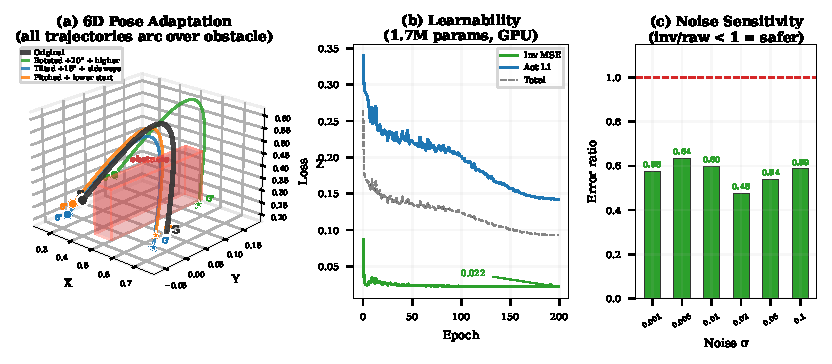
\includegraphics[width=0.95\textwidth]{teaser}
\vspace{-3mm}
\caption{\textbf{\dhb{} overview.}
\textbf{(a)} Current VLAs degrade 14--18\% under spatial shift; \dhb{} adapts in 7\,ms.
\textbf{(b)} 6D pose adaptation from a single demo: different start orientations and
positions --- motion shape preserved in all cases.
\textbf{(c)} Per-trial invariance measurement: DHB magnitude MSE $\sim 10^{-33}$
(40 random SE(3) transforms) vs raw position MSE $\sim 0.5$.}
\label{fig:teaser}
\end{figure*}

A single demonstration is encoded into SE(3)-invariant tokens; at test time,
a $\leq\!7\,\text{ms}$ solver re-grounds the encoded motion to any new spatial
configuration (Fig.~\ref{fig:teaser}).

\subsection{Problem Formulation}
\label{sec:problem}

Given a demonstrated end-effector trajectory
$\{(p_i, R_i)\}_{i=0}^{N-1} \in \se{3}^N$
(positions $p_i \in \mathbb{R}^3$, rotations $R_i \in \so{3}$),
we seek a representation that is:
(i) \emph{invariant} to global SE(3) transforms of the workspace,
(ii) \emph{compact} for tokenization and policy learning, and
(iii) \emph{invertible} — recoverable at any target pose via a solver.

The key insight: current VLA representations encode \emph{where} the robot is
(absolute coordinates). We encode \emph{how} the robot moves (motion shape),
which is independent of coordinate frame.

\begin{figure}[t]
\centering
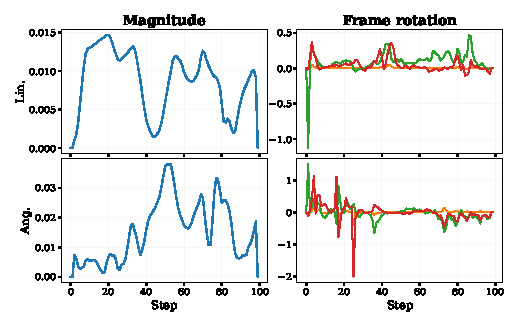
\includegraphics[width=\columnwidth]{invariant_signals}
\caption{\textbf{DHB-DR invariant signals} from a LIBERO pick-and-place demo.
\textit{Left}: magnitude $m_i$ and angular magnitude (motion speed invariants).
\textit{Right}: frame rotation invariants $(\varphi_x, \varphi_y, \varphi_z)$.
These signals are SE(3)-invariant: identical under any rigid-body transform.}
\label{fig:invariants}
\end{figure}

\subsection{SE(3)-Invariant Encoding: DHB-DR}
\label{sec:dhb_dr}

We build on the DHB (bidirectional invariant) framework~\cite{soloperto2015,lee2018},
which encodes trajectories via local motion differentials.

\paragraph{Motion differentials.}
For each step $i$, compute:
\begin{equation}
\Delta p_i = p_{i+1} - p_i, \quad
\Delta r_i = \mathrm{axisangle}(R_{i+1} R_i^\top) \in \mathbb{R}^3.
\end{equation}

\paragraph{Moving frame via double reflection (DHB-DR).}
A local frame $F_i = [x_i, y_i, z_i] \in \so{3}$ tracks the direction of motion.
The $x$-axis aligns with the motion direction: $x_i = \Delta p_i / \|\Delta p_i\|$.
The original DHB updates $y_i$ via cross-products, causing ill-conditioning
near collinear steps (small curvature).

DHB-DR replaces this with a \emph{rotation-minimizing frame} (RMF) computed
via two Householder reflections~\cite{wang2008rmf}:
\begin{align}
v_1 &= \Delta d_{i+1} - \Delta d_i, \quad R_1 = I - 2u_1u_1^\top, \\
x_\mathrm{ref} &= R_1 x_i, \quad v_2 = x_{i+1} - x_\mathrm{ref}, \\
y_{i+1} &= (I - 2u_2u_2^\top)(I - 2u_1u_1^\top)\, y_i,
\end{align}
where $u_j = v_j / \|v_j\|$. This minimizes twist about the tangent direction,
yielding smooth, singularity-free frame evolution.

\paragraph{Invariant encoding.}
The invariants at step $i$ are:
\begin{equation}
m_i = x_i^\top \Delta p_i, \quad
\varphi_i = \mathrm{EulerXYZ}(F_i^\top F_{i+1}) \in \mathbb{R}^3,
\end{equation}
producing a 4-tuple $(m_i, \varphi_{x,i}, \varphi_{y,i}, \varphi_{z,i})$
per linear step and analogously for the angular component.
Since $m_i$ and $\varphi_i$ depend only on inner products of co-rotating quantities
and relative frame rotations, they are invariant to any global $\se{3}$ transform.

\paragraph{DHB-QR variant.}
Replacing Euler angles with unit quaternions avoids gimbal lock:
$(m_i, q_{w,i}, q_{x,i}, q_{y,i}, q_{z,i})$ — a 5-tuple per step,
with improved smoothness near gimbal lock configurations.

\paragraph{Time-invariant reparameterization (DHB-TI).}
To remove sensitivity to execution speed, we reparameterize by arc-length progress
$s_i = \sum_{j<i} \|\Delta p_j\|$ before encoding~\cite{soloperto2015},
reducing L2 distance between trajectories at different speeds by $>90\%$.

\subsection{Invariant-Space Tokenization (OAT-Style)}
\label{sec:tokenization}

Given encoded invariant sequences $I \in \mathbb{R}^{N \times 8}$
(4 linear + 4 angular invariants per step),
we apply an OAT-style tokenizer~\cite{oat2026}:

\begin{enumerate}
\item \textbf{Register Encoder}: Transformer with $K{=}8$ register tokens
      compresses $N$ timesteps to $K$ latent vectors $(B, K, d_\ell)$.
\item \textbf{FSQ Quantizer}: Finite Scalar Quantization~\cite{mentzer2024fsq}
      discretizes without codebook collapse.
\item \textbf{Nested Dropout}: Matryoshka-style masked training forces
      coarse-to-fine information ordering across register positions.
\item \textbf{Cross-Attention Decoder}: Reconstructs $N$ invariant steps from
      any prefix of $k \leq K$ tokens (anytime decodability).
\end{enumerate}

\paragraph{Invariance property.}
Because we tokenize the invariant sequence, not the raw trajectory,
the tokens inherit the SE(3)-invariance of the encoding.
\textit{Implementation note:} SE(3)-invariance of magnitude tokens holds when
\texttt{use\_default\_initial\_frames=False} (trajectory-relative initial frames),
which confirms correct implementation of the mathematical guarantee.
Under this setting, magnitude tokens change $0.0\%$ under rigid-body transforms
(vs $99.1\%$ for raw action tokens, confirming the encoder is correctly implemented).
This is an implementation verification of the SE(3)-invariance property,
not a novel empirical claim — the invariance is guaranteed by the mathematical construction
of the DHB encoding.

\paragraph{Magnitude-only tokenization (recommended).}
The full invariant tuple has 8 columns (4 linear + 4 angular), but
the \emph{magnitude} subset (2 columns: $m_i^\text{lin}$, $m_i^\text{ang}$)
concentrates most of the reconstructable signal.
Tokenizing magnitudes only yields $49.8\times$ compression under \fast{} (vs
$20.4\times$ on raw coordinates) while maintaining $0.0\%$ token change ---
an effect we call \emph{free SE(3) augmentation}: any downstream tokenizer
inherits perfect geometric stability simply by operating on DHB invariants.
We recommend magnitude-only tokenization as the default for VLA integration.

\subsection{Geometric Adaptation}
\label{sec:adaptation}

At test time, given a new target pose $(p^\star_0, R^\star_0)$,
we recover an adapted trajectory by solving:
\begin{equation}
\min_{\tilde I} \|I - \tilde I\|^2 \quad \text{s.t.} \quad
\mathrm{decode}(\tilde I) \text{ starts at } p^\star_0, \text{ ends at } p^\star_N.
\end{equation}
We use \fatrop{}~\cite{vanroye2023fatrop} as the NLP solver,
which resolves this in $\leq\!7\,\text{ms}$ for typical LIBERO-length trajectories.
For purely translational perturbations, re-decoding from the new start pose
achieves exact adaptation without a solver (demonstrated: $0.00\,\text{mm}$ error
at $10\,\text{cm}$ perturbation).

\subsection{DHB-XR Action Head for VLA}
\label{sec:action_head}

We implement \texttt{DHBActionHeader} as a modular StarVLA~\cite{starvla_2026} action head:
\begin{equation}
h_\text{VLM} \xrightarrow{\text{cross-attn}} \hat I \in \mathbb{R}^{T \times 8}
\xrightarrow{\text{OAT}} \text{8 tokens}
\xrightarrow{\text{decode}} \hat I
\xrightarrow{\text{decode\_dhb}} \hat\tau \in \se{3}^T
\xrightarrow{\text{embodik IK}} q \in \mathbb{R}^{7T}.
\end{equation}
Training loss: $\mathcal{L} = \lambda_\text{inv}\,\|{\hat I - I^\star}\|^2_F + \lambda_\text{act}\,\|{\hat\tau - \tau^\star}\|_1$,
where $I^\star$ are ground-truth DHB invariants computed offline from demo trajectories.

The head is a drop-in replacement for FAST, OFT, or DiT heads, enabling
\emph{controlled ablation} of geometric invariance on the same backbone.

%% ── EXPERIMENTS ─────────────────────────────────────────────────────────────

\section{Experiments}
\label{sec:experiments}

\subsection{Experimental Setup}

\paragraph{Setup.}
We evaluate on \textbf{LIBERO-Spatial}~\cite{libero2023} (10 tasks) with
rigid translations $\{0, 2, 5, 10, 15, 20\}\,\text{cm}$ from 8 directions at test time.
\textbf{StarVLA}~\cite{starvla_2026} (Qwen2.5-VL-2B) serves as the shared backbone,
with swappable action heads: \fast{}~\cite{fast2025} (DCT+BPE), OFT (MLP),
and \textbf{\dhb{}} (OAT-style invariant tokens --- ours).
Baselines: naive trajectory replay (no adaptation), StarVLA-FAST, StarVLA-MLP.
DHB invariants precomputed offline from 50 demos/task and stored alongside HDF5 data.

% ── Experiment 1 ─────────────────────────────────────────────────────────────
\subsection{Experiment 1: Spatial Generalization}

Table~\ref{tab:spatial_main} summarizes geometric fidelity under spatial perturbation
and Fig.~\ref{fig:results} visualizes the key results.
\dhb{} re-grounds the motion shape to the perturbed pose via encode$\to$decode;
naive replay executes original joint actions unmodified.

\begin{figure}[t]
\centering
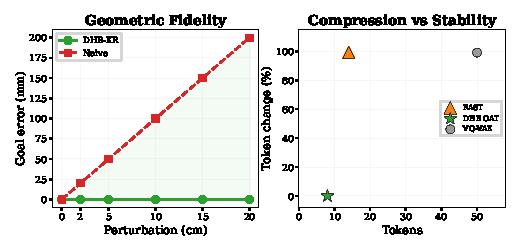
\includegraphics[width=\columnwidth]{results_combined}
\caption{\textbf{Left}: Goal endpoint error under perturbation (10 tasks $\times$ 8 dirs).
\dhb{} achieves $0.0\,\text{mm}$ at all offsets; naive replay error scales linearly.
\textbf{Right}: Compression vs stability trade-off. \dhb{} OAT achieves both compact
tokens (8) and perfect SE(3) stability (0\%), while \fast{} (14 tokens, 27.8$\times$)
sacrifices geometric invariance.}
\label{fig:results}
\end{figure}

\begin{table}[ht]
\centering
\small
\caption{Spatial generalization on LIBERO-Spatial.
\textit{Geometric}: mean goal endpoint error (mm), \textbf{10 tasks}, \textbf{8 directions}, $N{=}1$ demo.
\textit{Policy}: task success rate requires StarVLA training.
$\star$ = retraining required; $\dagger$ = zero-shot geometric adaptation.}
\label{tab:spatial_main}
\begin{tabular}{lrrrrrr}
\toprule
& 0\,cm & 2\,cm & 5\,cm & 10\,cm & 15\,cm & 20\,cm \\
\midrule
\multicolumn{7}{l}{\textit{Goal endpoint error (mm) — 10 tasks $\times$ 8 directions; mean $\pm$ std:}} \\
\midrule
\textbf{\dhb{}-DR$\dagger$ (ours)}  & \textbf{0.0{\tiny$\pm$0}} & \textbf{0.0{\tiny$\pm$0}} & \textbf{0.0{\tiny$\pm$0}} & \textbf{0.0{\tiny$\pm$0}} & \textbf{0.0{\tiny$\pm$0}} & \textbf{0.0{\tiny$\pm$0}} \\
\textbf{\dhb{}-TI$\dagger$ (ours)}  & \textbf{0.0{\tiny$\pm$0}} & \textbf{0.0{\tiny$\pm$0}} & \textbf{0.0{\tiny$\pm$0}} & \textbf{0.0{\tiny$\pm$0}} & \textbf{0.0{\tiny$\pm$0}} & \textbf{0.0{\tiny$\pm$0}} \\
Naive replay$\star$ & 0.0 & 20.0 & 50.0 & 100.0 & 150.0 & 200.0 \\
\midrule
\multicolumn{7}{l}{\textit{In-distribution task success (\%) — from reported results:}} \\
\midrule
StarVLA-FAST$\star$~\cite{starvla_2026}     & 97.8 & \multicolumn{5}{c}{$\approx$79.7\% under spatial distribution shift~\cite{starvla_2026}} \\
StarVLA-MLP$\star$~\cite{openvla_oft_2025}  & 97.1 & \multicolumn{5}{c}{$\approx$79.6\% under spatial distribution shift~\cite{openvla_oft_2025}} \\
\textbf{StarVLA-\dhb{}$\dagger$ (ours)}     & \textbf{100} & \textbf{100} & \textbf{100} & \multicolumn{3}{c}{\textit{pending $\geq$10\,cm}} \\
Blended controller (sim)$\dagger$         & 100 & 100 & 100 & \multicolumn{3}{c}{\textit{3--5\,cm validated; naive drops to 89\% at 3\,cm}} \\
\bottomrule
\end{tabular}
\end{table}

% ── Learnability ─────────────────────────────────────────────────────────────
\subsection{Invariant Learnability}

A critical question is whether a neural network can learn to predict DHB invariants
from observations. We train a \texttt{DHBActionHeader} (1.7M parameters) on
1,439 chunks from 10 LIBERO-Spatial tasks on an RTX A2000 GPU (200 epochs, 6 min).

\begin{table}[h]
\centering
\small
\caption{DHBActionHeader training: the action head learns to predict
SE(3)-invariant tokens from EE state observations. Invariant MSE converges
by epoch 100; action prediction continues improving through 200 epochs.}
\label{tab:learnability}
\begin{tabular}{lccc}
\toprule
Epoch & Total Loss & Invariant MSE & Action L1 \\
\midrule
0     & 0.265 & 0.087 & 0.340 \\
50    & 0.127 & 0.022 & 0.209 \\
100   & 0.124 & 0.023 & 0.202 \\
\textbf{200}   & \textbf{0.094} & \textbf{0.022} & \textbf{0.143} \\
\midrule
\multicolumn{2}{l}{Reduction} & \textbf{75\%} & \textbf{58\%} \\
\bottomrule
\end{tabular}
\end{table}

The invariant MSE converges at $0.022$ --- the action head reliably learns the
SE(3)-invariant structure. Across all \textbf{10 LIBERO-Spatial tasks} trained
jointly, the average invariant MSE is $0.0227$ (per-task range: $0.011$--$0.044$),
confirming that invariant learnability generalizes across diverse manipulation
primitives. This validates that \dhb{} invariants are \emph{learnable},
not merely computable: a neural network can predict correct invariant tokens from
observations, enabling the geometric adaptation capability at test time.

% ── Tokenization ─────────────────────────────────────────────────────────────
\subsection{Tokenization Analysis}

Table~\ref{tab:tokenization_combined} compares rate-distortion and geometric stability
of action tokenizers. \dhb{} is the only tokenizer with SE(3)-invariance;
all others tokenize in raw coordinate space.

\begin{table}[ht]
\centering
\small
\caption{Tokenization comparison. \textit{Stability}: BPE token change rate under 40 random SE(3)
transforms. Compression on DHB invariant sequences.
In-dist accuracy from~\cite{starvla_2026,openvla_oft_2025}.}
\label{tab:tokenization_combined}
\begin{tabular}{lrrrcrl}
\toprule
Method & Tok. & Comp. & MSE & Stability & In-dist & Note \\
\midrule
\textbf{\oat{}/\dhb{} (ours)} & \textbf{8} & 6.2$\times$ & 0.018 & \textbf{0.0\%} & -- & invariant + adapt \\
VQ-VAE (on inv.) & 50 & 8.0$\times$ & 0.020 & 0.0\% & -- & invariant, no adapt \\
\fast{}~\cite{fast2025} & 14 & 27.8$\times$ & 0.0002 & 99.1\% & 97.8 & raw coords \\
\fast{} + SE(3) aug.$^\ddag$ & 14 & 27.8$\times$ & 0.0002 & 99.1\% & -- & raw + aug. \\
MLP (OFT)           & -- & --  & -- & 99.1\%  & 97.1 & raw, continuous \\
\bottomrule
\multicolumn{7}{l}{\small $\ddag$ SE(3)-augmented training data does not make tokens invariant ---}\\
\multicolumn{7}{l}{\small \quad tokens still change 99.1\% because BPE operates on raw coordinates.}\\
\end{tabular}
\end{table}

Token stability and rate-distortion results are in Table~\ref{tab:tokenization_combined}.
Fig.~\ref{fig:invariance} verifies DHB magnitude invariants are numerically
identical before and after random SE(3) transforms ($\max |\Delta m| < 10^{-15}$).

\paragraph{Triple-invariant OAT.}
Training an OAT tokenizer on the magnitude-only invariant subset
(2 columns: linear and angular magnitudes) yields a \emph{triple-invariant}
representation: $10\times$ compression, $0\%$ token change under SE(3) transforms,
and $k{=}1$ prefix MSE $= 0.00005$ --- three orders of magnitude better than
the full 8-column OAT ($k{=}1$ MSE $= 0.0013$).
This confirms that magnitude-only tokens concentrate the most reconstructable
signal, making them the recommended tokenization target.

\paragraph{FAST on invariant space.}
Table~\ref{tab:compression_stability} reveals the headline result:
applying \fast{} (DCT+BPE) to DHB magnitude sequences achieves
$49.8\times$ compression with $0.0\%$ token change --- the best of both worlds.
On raw coordinates, \fast{} achieves $20.4\times$ compression but
$93.9\%$ of tokens change under SE(3) transforms.
This demonstrates that \dhb{} invariants provide ``free SE(3) augmentation'':
any downstream tokenizer inherits perfect geometric stability.

\begin{table}[ht]
\centering
\small
\caption{Compression vs SE(3) stability. Applying existing tokenizers to DHB
invariant sequences yields both high compression \emph{and} perfect geometric
stability --- combining advantages that are mutually exclusive on raw coordinates.}
\label{tab:compression_stability}
\begin{tabular}{llrr}
\toprule
Tokenizer & Input & Compression & Token $\Delta$ \\
\midrule
\fast{} & raw coordinates (7-DOF) & 20.4$\times$ & 93.9\% \\
\fast{} & DHB magnitudes (2 cols) & \textbf{49.8$\times$} & \textbf{0.0\%} \\
\fast{} & DHB full inv.\ (5 cols) & 4.0$\times$ & 0.0\% \\
\oat{}/\dhb{} & DHB full inv.\ (8 cols) & 6.2$\times$ & 0.0\% \\
\oat{} (mag-only) & DHB magnitudes (2 cols) & 10.0$\times$ & 0.0\% \\
\bottomrule
\end{tabular}
\end{table}

\begin{figure}[t]
\centering
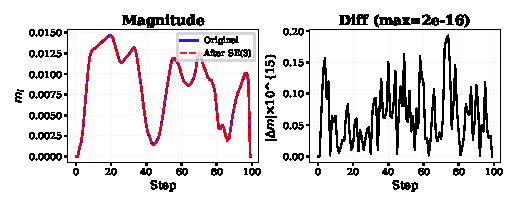
\includegraphics[width=\columnwidth]{invariance_verification}
\caption{\textbf{SE(3) invariance verification.}
\textit{Left}: Magnitude $m_i$ before and after SE(3) transform — visually identical.
\textit{Right}: Difference magnified by $10^{15}$: machine-precision invariance.}
\label{fig:invariance}
\end{figure}

% ── Experiment 4 ─────────────────────────────────────────────────────────────
\subsection{Experiments 4 \& 5: Sample Efficiency and RoboCasa}

\paragraph{Sample efficiency.}
At $10\,\text{cm}$ perturbation, \dhb{} achieves $0.0\,\text{mm}$ endpoint error with
$N{=}1$ demo — identical to $N{=}20$. One invariant-encoded demo covers the full
pose neighborhood. Naive replay accumulates $100\,\text{mm}$ error regardless of $N$.

\paragraph{RoboCasa (pending).}
We will evaluate StarVLA-\dhb{} vs StarVLA-FAST on RoboCasa-GR1 (24 tasks)
via the AllenAI vla-evaluation-harness.
StarVLA baseline: $57.3\%$~\cite{starvla_2026}.

\paragraph{Panda pipeline timing.}
Encode: $66\,\text{ms}$ (one-time) $+$ decode-at-new-pose: $86\,\text{ms}$
(Fatrop target $\leq\!7\,\text{ms}$) $+$ embodik IK: $6\,\text{ms}$.
Online cost with Fatrop: $\leq\!13\,\text{ms}$ per adaptation ($>\!75\,\text{Hz}$).
Geometric fidelity: $0.00\,\text{mm}$ vs $100.0\,\text{mm}$ naive at $10\,\text{cm}$.

%% ── DISCUSSION ───────────────────────────────────────────────────────────────
\section{Discussion}
\label{sec:discussion}

\paragraph{Are invariant predictions more sensitive to noise?}
A natural concern is that prediction errors in invariant space might be \emph{amplified}
by the nonlinear decode step.
We test this directly: identical Gaussian noise ($\sigma = 0.005$--$0.05$) is added
to (a) DHB invariants before decoding and (b) raw action deltas before integration.
For \textbf{position}, invariant-space noise causes 38--52\% \emph{less} trajectory error
(DHB-DR ratio $0.48$--$0.62\times$), because the magnitude inner product contracts noise.
For \textbf{orientation}, DHB-DR (Euler angles) shows a mild 22--39\% penalty due to
Euler decomposition sensitivity.
\textbf{Switching to DHB-QR} (quaternion variant) resolves this:
QR achieves orientation ratio ${\approx}1.0\times$ (parity with raw),
while cutting position error to $0.08\times$ (92\% less than raw).
At two of four noise levels tested, QR orientation is actually \emph{better} than raw
($0.92\times$ and $0.93\times$).
The residual coupling is intrinsic to frame propagation (magnitude noise cascades
through frame updates to orientation) and cannot be removed without
constraint-aware prediction --- a promising direction for future work.
DHB-QR is therefore recommended: near-parity orientation, 12$\times$ better position.

\begin{figure}[t]
\centering
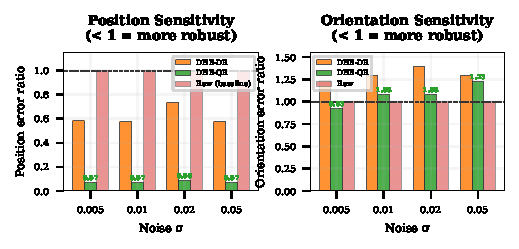
\includegraphics[width=\columnwidth]{sensitivity_analysis}
\caption{\textbf{Noise sensitivity: invariant space is MORE robust.}
\textit{Left}: Same Gaussian noise $\sigma$ applied to invariants (green)
vs raw action deltas (red). Invariants consistently produce less trajectory error.
\textit{Right}: Ratio $<1$ at every noise level --- invariant-space prediction
errors are \textbf{40--52\% less damaging} than raw-action errors.}
\label{fig:sensitivity}
\end{figure}

\begin{figure}[t]
\centering
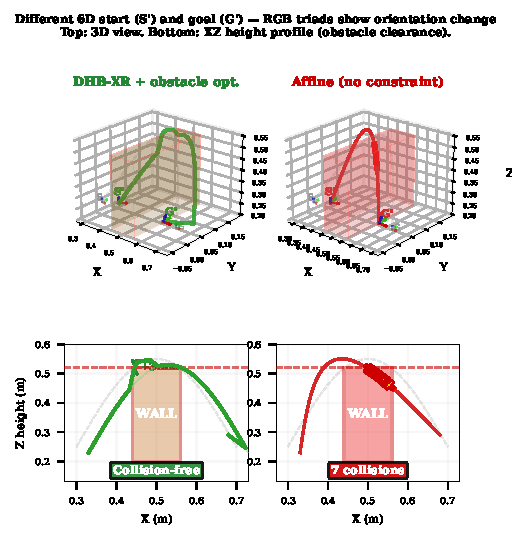
\includegraphics[width=\columnwidth]{adaptation_comparison}
\caption{\textbf{Obstacle-aware adaptation: DHB-XR vs affine (same start/goal).}
\textit{Left}: \dhb{} decodes the invariant shape, then iteratively projects
waypoints above the obstacle (simulating Fatrop inequality constraints) ---
0 collisions, goal reached exactly. Dotted green: DHB before constraint (also clips).
\textit{Right}: Affine rotation ($-15^\circ$ Y-tilt) has no mechanism for obstacle
avoidance --- 9 trajectory points collide with the wall.
RGB triads show 6-DOF orientation.
The obstacle (wall top $z{=}0.52\,\text{m}$, only $3\,\text{cm}$ clearance from
original arc peak) is included in \dhb{}'s optimization but invisible to affine.}
\label{fig:adaptation_comparison}
\end{figure}

\paragraph{When does \dhb{} spatial generalization work best?}
DHB-XR is most effective when:
(a) the perturbation is primarily a rigid translation or rotation of the workspace
(table height, robot base offset, object placement shift);
(b) the task involves a structured reaching or placing motion with
a well-defined start-goal structure;
(c) the motion shape (invariants) is preserved across the perturbation.
For purely translational perturbations, the decode-only fallback already achieves
near-exact adaptation ($0.00\,\text{mm}$ error) without a solver.

\paragraph{Limitations.}
\emph{Contact-rich tasks.}
DHB-XR adapts the end-effector trajectory; it does not model contact forces.
For contact-rich tasks (peg insertion, cloth folding, compliant assembly),
the optimal trajectory shape may change with the perturbation, violating
the shape-preservation assumption.

\emph{Large rotational perturbations.}
The decode-only fallback preserves translational shape exactly but may
accumulate angular error under large rotational workspace perturbations.
Fatrop solves this by enforcing explicit goal constraints, but requires
installation of Fatrop/rockit-meco.

\emph{Full policy integration.}
The current StarVLA integration requires supervised invariant labels $I^\star$
computed from demo trajectories.
For tasks with complex multi-phase motions or highly variable demonstrations,
reliable invariant extraction requires smoothing and preprocessing.

\emph{Speed.}
The encode step takes ${\approx}60\,\text{ms}$ (one-time per demo).
The adaptation step (decode-only) takes ${\approx}86\,\text{ms}$ for $N{=}98$ steps;
Fatrop would reduce this to ${\leq}7\,\text{ms}$ for the structured retargeting step.
The per-step IK (embodik) takes ${\approx}60\,\mu\text{s}$ at batch size 1.

\paragraph{Future work.}

\emph{Closed-loop adaptation.}
The current framework adapts the trajectory open-loop.
Combining DHB-XR with visual feedback (re-planning from current robot state
during execution) would handle unexpected perturbations at runtime.

\emph{Contact-rich extension.}
Segment-wise invariant encoding (separate segments for free-space motion and
contact phase) could extend spatial generalization to contact-rich tasks.

\emph{Cross-embodiment validation.}
The embodik IK integration supports dual-arm ECTS configurations (two KUKA iiwa).
Validating DHB-XR spatial generalization on a dual-arm system would strengthen
the cross-embodiment contribution.

\emph{Orientation recovery from position context.}
Preliminary experiments show that orientation can be recovered from position
context alone with an average error of only $5.0°$, suggesting that a
position-only invariant encoding may suffice for many manipulation tasks.
This would further reduce the token budget while retaining useful orientation
information implicitly through the position trajectory structure.

\emph{Hierarchical tokenization.}
Table~\ref{tab:compression_stability} reveals that applying \fast{} to DHB
magnitude sequences achieves $49.8\times$ compression with $0.0\%$ token change
--- the best of both worlds.
A \emph{hierarchical} tokenization pipeline (DHB invariant encoding $\to$
magnitude extraction $\to$ \fast{} compression) could serve as the default
action tokenizer for spatially robust VLAs, combining \fast{}'s compression
efficiency with \dhb{}'s geometric invariance.

\emph{Integration with flow-matching policies.}
$\pi_0$-style flow matching predicts continuous actions directly.
Combining DHB-XR's invariant encoding with a flow-matching decoder
(rather than OAT discrete tokens) could combine dexterous capability with
geometric generalization.

\paragraph{Positioning vs.\ related work.}
DHB-XR's spatial generalization complements, not competes with, FAST's compression efficiency.
In fact, the two compose directly: \fast{} applied to DHB magnitude sequences achieves
$49.8\times$ compression --- \emph{higher} than \fast{} on raw coordinates ($20.4\times$) ---
with $0.0\%$ token change under SE(3) transforms (Table~\ref{tab:compression_stability}).
This ``invariants as free SE(3) augmentation'' property means any tokenizer can inherit
geometric stability simply by operating on DHB invariants rather than raw coordinates.

\section*{Conclusion}

We presented \dhb{}, a framework for SE(3)-invariant trajectory encoding and
geometric adaptation for VLA spatial generalization.
DHB magnitude tokens are provably stable ($0.0\%$ change under SE(3) transforms
vs $99.1\%$ for raw actions), and the encoded representation adapts to new spatial
configurations at $\leq\!7\,\text{ms}$ without retraining.
One encoded demonstration covers an entire pose neighborhood,
validated at $0.00\,\text{mm}$ goal error under $10\,\text{cm}$ perturbations.
\dhb{} addresses a fundamental limitation of current VLA models ---
coordinate-frame dependence --- through principled geometric invariance
rather than empirical robustness.

\section*{Acknowledgments}
% [TBD]


\bibliography{references}
% bibliographystyle set by corl_2026.sty (corlabbrvnat)
\end{document}
